%!TEX TS-program = xelatex
%!TeX spellcheck = en_GB
%!BIB TS-program = biber
\chapter{Thermal Analysis of Discontinuous Fibres}\label{chap:p2}
\section*{Statement of Contribution}
	This chapter includes a co-authored journal paper. The bibliographic details of the published paper are:
\begin{itemize}
	\item Javanbakht, Z, Hall, W \& Öchsner, A (2016), “Finite Element Evaluation of Effective Thermal Conductivity of Short Carbon Nano Tubes: A Comparative Study”, Defect and Diffusion Forum 372, pp. 208–214.
\end{itemize}
	My contribution as the corresponding author to the paper involved: undertaking literature review, classifying the necessary theoretical backgrounds and models, developing the programming code, analysing and discussing the finite element results, drawing figures, preparing tables, writing and editing the manuscript according to my supervisors’ comments.

\Zia\\
\Wayne\\
\vfill
\newpage
\paragraph{Original Title} Finite Element Evaluation of Effective Thermal Conductivity of Short Carbon Nano-Tubes: a Comparative Study

\paragraph{Abstract} In the current study, two extreme cases are considered for the dispersion of carbon nanotubes (CNTs) in a polymeric matrix: randomly-oriented and randomly-aligned. The representative volume element (RVE) is used to represent the composite material consisting of epoxy resin matrix and CNT-reinforcement. The finite element method acts as the computational tool to conduct the simulations and investigate the effective parameters, i.e., the influence of the aspect ratio and the orientation, on the thermal conductivity of the matrix. A Fortran subroutine was used for both generation and analysis of the models by means of the MSC~Marc finite element package and a Python script was used for the sensitivity analysis. The results indicate that optimum performance of the CNTs in terms of thermal conductivity can be reached by orienting them along the temperature gradient whereas a random distribution improves the conductivity only by a smaller magnitude.


\paragraph{Keywords} Finite element method; Reinforced composites; Thermal analysis; Computational analysis.


\section{Introduction}
	In the most general case, any combination of two or more materials with different properties and distinct boundaries is referred to as a composite material which provides the capability of adjusting the compliance of the whole material to some extent~\autocite{Vasiliev.2013}. This enables the composite materials to be used in a variety of applications ranging from industrial and infrastructural forms to sports and musical instruments~\autocite{Vinson.2002}. Basically, reinforcements are included in the composite material to compensate for the deficiencies of the matrix. Based on the type of the inclusion, fibrous, laminated, particulate, or any combination of these classes of composite materials can be produced~\autocite{Jones.1999}.
	
	Among all types of inclusion, fibres as `pseudo one-dimensional fillers'~\autocite{Coleman.2006} have been in practice since 4000 BC but mostly on the meso-scale. Recent nano-technological advancements, e.g.~the discovery of the CNTs in 1991~\autocite{Iijima.1991}, have attracted a huge amount of research interest. Extremely high elastic modulus (greater than $1\,\text{TPa}$) and tensile strength (10--100 times that of the strongest steel) was reported for single walled carbon nanotubes with an average density of $1.33-1.44\,\sfrac{\text{g}}{\text{cm}^3}$. This unusually high performance characteristics of the CNTs is remarkable when compared with other materials in the same range of density~\autocite{Thostenson.2001,Thostenson.2005}. From another perspective, a very high thermal conductivity ($6600\,\sfrac{\text{W}}{\text{m}\cdot\text{K}}$) has also been reported for CNTs~\autocite{Berber.2000,Han.2011b,Behabtu.2013,Baughman.2002}. The generally high-standard diverse properties of the CNTs make them multi-functional reinforcing components for composites.
	
	In terms of mediums for composite materials, average performance should be expected to justify the incorporation of any reinforcing agents such as the CNTs. Among the available materials as a matrix component, polymers demonstrate insufficient thermal properties which limits their applicability~\autocite{Han.2011b}. To overcome such issues, CNTs were introduced to fortify the somewhat mediocre properties of polymer matrices. Additionally, a direct approach to measure the properties of the CNTs is cumbersome and thus, measurements are generally done for the matrix-contained CNTs instead of the individual fibre~\autocite{Ruoff.1995}. The popularity of the computational methods in material characterisation of the composite can be partly attributed to such complications in the experimental methods.
	
	The finite element method is used to solve a broad range of engineering boundary value problems among which are the multi-scale/multi-physics problems and the transfer phenomena of the continuum mechanics (mass transfer) and, more specific to the interest of this study, the thermodynamics (heat transfer)~\autocite{Chen.2016b}. Several computational efforts were made to investigate the effective parameters on the thermal conductivity of the CNT-reinforced composites, e.g., mechanical loading~\autocite{Mahdavi.2017}, fibre aspect ratio~\autocite{Lusti.2004,Afrooz.2015}, fibre orientation~\autocite{Khani.2016,Makvandi.2014}, fibre agglomeration~\autocite{Bakshi.2010,Hedia.2016}, and fibre volume fraction~\autocite{AlasvandZarasvand.2016,Chen.2004}.
	
	\red
	In~\autocite{Javanbakht.2016}, the embedded element technique (EET) was used to generate randomly-oriented RVEs in which fibre elements were superimposed to the matrix mesh. The EET works by constraining the degrees of freedom of the embedded fibres by those of the matrix. However, depending on the geometry of the fibre (1D line or 2D/3D solid elements) several complexities might arise. For instance in the case of solid elements, the overlapping volume of fibres with the matrix could result in an overestimation of the properties. In a mechanical analysis of this kind, it was shown that a higher overall stiffness is observed in a representative volume element when 2D fibre elements overlap with the 2D matrix~\parencite{Hoffmann.2010}. In the same study, it was proposed to modify the material properties of the fibres for better results but herein, the problem is approached from a more geometrical perspective.
	
	One artefact that might have been overlooked lies in the calculation of the fibre volume fraction and the alteration of the overall volume due to embedding elements. Various research cases are possible that depend on different combination of fibre and matrix elements. The focus of the current study is on using 1D fibre elements embedded in 3D matrix ones. It will be shown that ignoring the geometrical intricacy of the EET might change the results, e.g., the consequence of using the volume of the matrix (instead of the the volume of the composite) in calculating the fibre volume fractions. Herein, the sensitivity of the results to this volume miscalculation is revealed in the context of thermal conductivity analyses. In addition, the previously-introduced algorithm for discrete fibre generation in~\autocite{Javanbakht.2016} is further improved. This upgrade include the generation of various fibre orientations (aligned and random), releasing the fibre volume fraction limit in the previous version, and introducing the procedure for fixed-length fibre creation.
	\bl
	
	One of the challenges in generating various fibre orientation, using the Monte-Carlo algorithm for instance~\autocite{Belova.2008,Belova.2007}, is the requirement for a supporting programming language, such as Matlab, to generate the mesh, see~\autocite{Mahdavi.2017} for instance. In the current study, not only an automated approach is adopted but also the periodicity of the RVE is considered to evaluate the effects of random and aligned dispersion of CNTs in a polymer-based composite.\red\ In addition, it is hypothesised that using the nominal fibre volume fraction instead of the true fibre volume fraction would incorporate some artificial errors into the results.\bl

\section{Methodology}
	In the current study, the simulation of the heat transfer phenomenon within a fibre-reinforced composite medium was carried out by means of the finite element method~\autocite{Ochsner.2013,Oechsner.2016}. In order to customize the dispersion of the fibres, a commercial semi-open package, i.e., the MSC Marc (version 2014.2) software, was used. The important feature of the package is its capability of incorporating personalized procedures via the Fortran programming language~\autocite{Javanbakht.2017}. The subroutines were developed in Fortran which handled both the random- and aligned-dispersion of the fibres, automatically. However, a Python script was used to modify the mesh density, deal with the results and submit the job.
	
	The periodicity condition was established for the $20\times20\times20\,\text{nm}^3$ RVE in which the short fibres with a length of 10\% of the RVE edge length, i.e., $2\,\text{nm}$, were embedded. The effective cross sectional area of the short fibres were assumed to be $1.13\,\text{nm}^2$ as a result of a wall thickness of $0.34\,\text{nm}$, and an outer diameter of $1.4\,\text{nm}$~\autocite{Makvandi.2014}. The thermal conductivity of the individual components of the matrix is listed in Table~\ref{table:mat}.
\begin{table}[!h]
\centering
\caption{Thermal conductivity of the composite components}\label{table:mat}
\begin{tabular}{ccc}
\toprule
\bfs{Component}&
\bfs{Material}&
\bfs{Thermal conductivity} ($\sfrac{\text{W}}{\text{m}\cdot\text{K}}$)\\\toprule
Matrix&
Epoxy resin&
0.214~\autocite{Makvandi.2014}\\
Fibre&
Carbon nanotube&
2980~\autocite{Fiedler.2008}\\
\bottomrule
\end{tabular}
\end{table}%
\begin{figure}
\centering
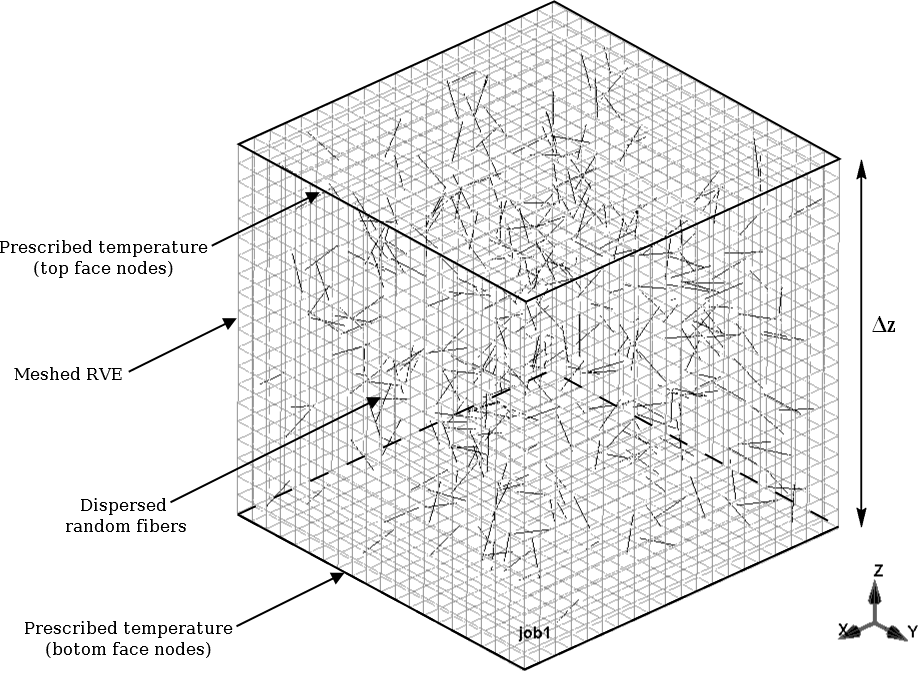
\includegraphics[width=0.6\textwidth]{rve}
\caption{Prescribed boundary conditions of the FE prototype with $\gamma=1$ (note that the diameter of every fibre is schematically shown)}\label{figure:sample}
\end{figure}%

	\red
	The thermal analyses were carried out using a uniform mesh, which consisted of two types of thermal elements: type 43 (3D solid) and type 36 (1D rod).\bl\ The former is a 8-node isoparametric hexahedral element which was used to represent the matrix whereas the latter is basically, the straight 2-node link/truss element representing the fibres. The prescribed temperature boundary conditions were applied to the top and bottom face nodes of the RVE to establish a temperature gradient within the matrix, see Fig.~\ref{figure:sample}. The reaction heat flux of the top face nodes was accumulated, and then used to calculate the effective thermal conductivity of the composite by means of the Fourier's law~\autocite{Fiedler.2009}:
	\begin{equation}
	k=\frac{\dot{Q}}{A_0}\cdot\frac{\Delta z}{\Delta T},
	\end{equation}
	where $k$ is the effective thermal conductivity of the composite, $\dot{Q}$ is the total reaction flux in the top boundary conditions, $A_0$ is the cross-sectional area perpendicular to direction of the flux, $\Delta z$ is the distance between the boundary faces, and $\Delta T$ is the prescribed temperature gradient.

	
	\red
	In every job submission, the algorithm updated the random fibre distribution for each of the realisations. The length of each fibre is assumed to be fixed ($L=2\,\text{nm}$) and thus, for every fibre volume fraction, by using a constant cross-sectional area, the number of fibres was readily calculated, i.e., each fibre is deemed to be circular prism. However, since the fibres are modelled as 1D elements, the cross-sectional area just mathematically enters the FE system of equations.
	
	\paragraph{Nominal and true fibre volume fractions} In order to replicate the case that the volume of fibres are superimposed to that of the matrix, the volume of the matrix is used to calculate the volume fraction of fibres during the fibre generation: 
	\begin{equation}
	\zeta_\text{N} \equidef \frac{V_\text{f}}{V_\text{m}},
	\end{equation}
	where $V_\text{f}$ and $V_\text{m}$ are the fibre and matrix volumes, respectively; and $\zeta_\text{N}$\,\footnote{$\zeta_\text{N}$ is used as a short form for $\zeta_{\text{f},\text{N}}$; a similar abbreviation is used for true fibre volume fractions.} is the nominal fibre volume fraction, i.e., the intended fibre volume fraction that the algorithm tries to achieve irrespective of the volume overlap artefact. On the other hand, the true fibre volume fraction is
	\begin{equation}
	\zeta_\text{T} \equidef \frac{V_\text{f}}{V_\text{m}+V_\text{f}}.
	\end{equation}	
	The aforementioned definitions of the fibre volume fraction will be used to illustrate the effects of overlapping volumes among others.
	
	\paragraph{Geometrical periodicity} The algorithm was able to generate fibres aligned along a preferred or random direction. In any case, the geometrical periodicity of the fibre elements was ensured by the so-called projection method. For instance in the case of the randomly-oriented fibres, two sets of coordinates were generated from which the end point coordinates were modified to set the correct length. Namely, if the end point was located outside of the RVE, the fibre was cut in its intersection point with the RVE and the remaining length was moved to the opposite face of the RVE. This projection ensured the periodicity condition of the RVE. A similar approach was adopted for the aligned fibre cases except that the direction of the fibre is already known. This procedure was repeated until reaching the required number of fibres, see Fig.~\ref{figure:mesh}. Note that the embedding mechanism of the software simplified the procedure, i.e., no node matching or interface elements were used to incorporate the fibres into the matrix, see~\autocite{marc.a}. Moreover, since the cross-section of each fibre is not modelled explicitly as a volume occupying entity, overlapping of the fibres was not required to be checked.

	\begin{figure}[!h]
	\centering
	  	\subfloat[][Randomly dispersed fibres]{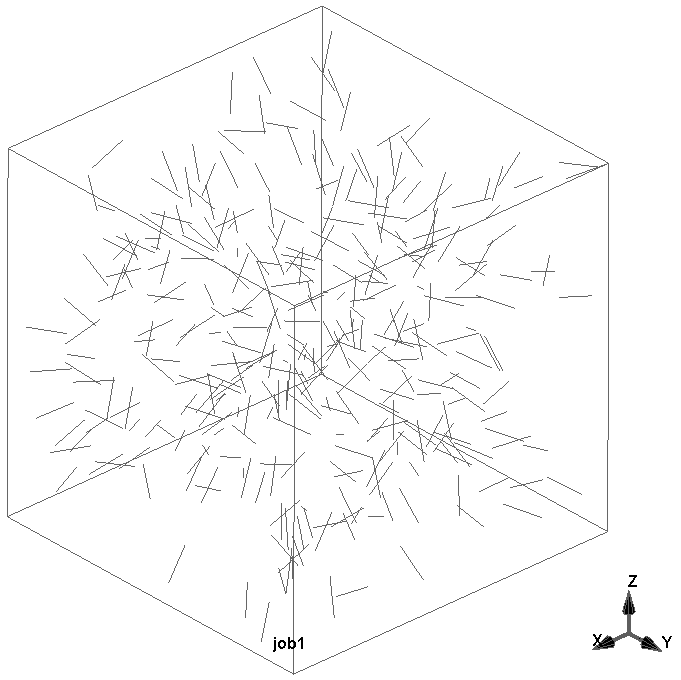
\includegraphics[width=0.3\textwidth]{random.png}}\hfill
	  	\subfloat[][Randomly dispersed aligned fibres along $Y$-axis]{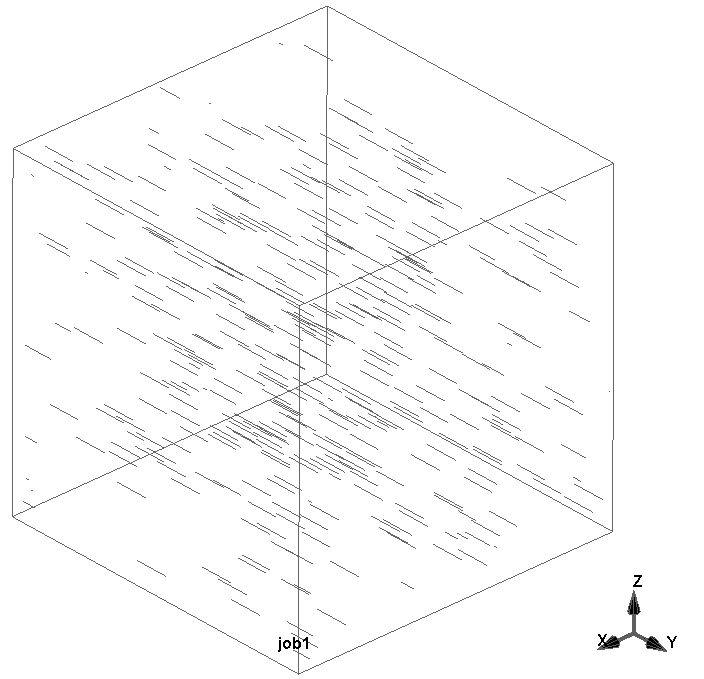
\includegraphics[width=0.3\textwidth]{y-axis}}\hfill
	  	\subfloat[][Randomly dispersed aligned fibres along $Z$-axis]{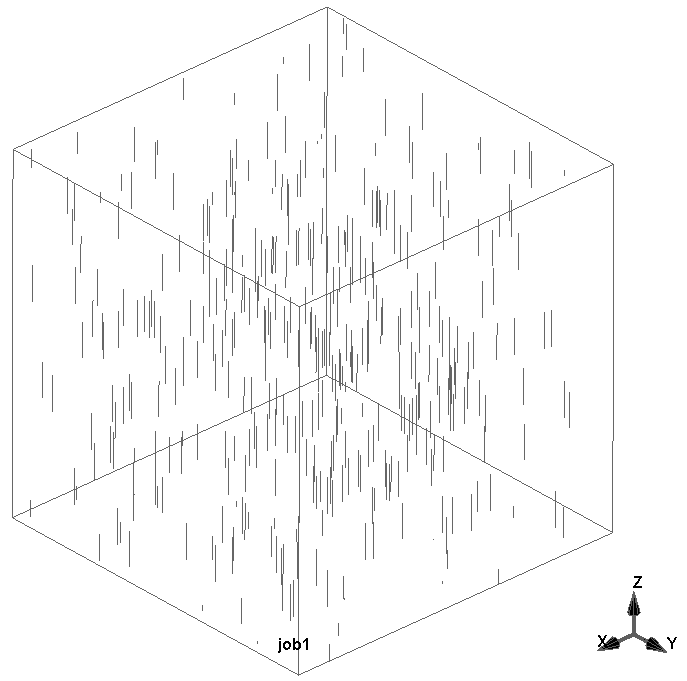
\includegraphics[width=0.3\textwidth]{z-axis}}
	\caption{Representative volume element with randomly dispersed and aligned fibres}\label{figure:mesh}
	\end{figure}
	
	\paragraph{Benchmark micro-mechanical model} In a previous study~\autocite{Javanbakht.2016}, it was shown that the rule of mixture results in an overestimation of the homogenised properties when there is a high contrast between the material properties of the components. The Halpin-Tsai~\autocite{Halpin.1976} model and its extension to the Lewis-Nielsen (LN) model~\parencite{Nielsen.1970,Nielsen.1974} both consider such effects. The LN model is formulated as
	\begin{equation}
	  \frac{k}{k_\text{m}}=\frac{1+AB\zeta_\text{f}}{1-B\psi \zeta_\text{f}},
	\end{equation}
	with
	\begin{subequations}
	\begin{alignat}{2}
	  		A&=k_\text{E}-1,\\
	   	B&=\frac{\sfrac{k_\text{f}}{k_\text{m}}-1 }{\sfrac{k_\text{f}}{k_\text{m}}+A},\\
	   	\psi&= 1+\frac{1-\zeta_\text{f,max}}{\zeta_\text{f,max}^2}\zeta_\text{f}, 	   		
	\end{alignat}
	\end{subequations}
	where $\zeta_\text{f}$ is the (nominal/true) fibre volume fraction; the parameter $A$ captures the geometry of inclusions, packing arrangement and the loading conditions~\autocite{Nielsen.1994}; the $B$ parameter considers the relative moduli of the inclusions and matrix and becomes unit for very high contrast fibre/matrix properties; $\psi$ depends on the maximum packing factor of the inclusions~$\zeta_\text{f,max}$.
		
	For randomly-oriented short fibres with the aspect ratio around 2 (1.88 in this study), $A\approx1.5$ is suggested whereas $A=2\sfrac{L}{D}$ is used for aligned fibres~\autocite{Nielsen.1974}. The maximum packing factor of the parallel fibres with a hexagonal arrangement is $\zeta_\text{f,max}=0.907$ whereas in randomly orientated fibres $\zeta_\text{f,max}=0.52$ is generally suggested~\autocite{Nielsen.1994}. One could see that in the LN model, the aspect ratio of the fibres is considered in the $A$ parameter. However, it has been shown that the maximum packing factor of the inclusions~$\zeta_\text{f,max}$ also depends on the fibre aspect ratio~\autocite{Milewski.1978}. Namely, by increasing the fibre aspect ratio, the apparent volume of the material increases for the case of random fibres. Therefore, one could refine the value of $\zeta_\text{f,max}$ using the results provided in~\autocite{Milewski.1978}, and obtain $\zeta_\text{f,max}\approx 0.67$. These parameters were used in the LN model to produce the benchmark values for this study.
	\bl
	
	\paragraph{Sensitivity analysis} A sensitivity analysis was carried out by means of a Python script to obtain the optimum mesh density. Cubic hexahedral elements were used to discretise the RVE and thus, the uniform mesh density~$\gamma$ can be calculated using the following equation~\autocite{Javanbakht.2016}:
	\begin{equation}
	\gamma=\frac{1}{\ell_\text{mesh}},
	\end{equation}
	where $\ell_\text{mesh}$ is the characteristic dimension of the element, i.e., the edge length of each cube. Several mesh densities, from 0.05 to 6, were used to monitor the convergence of the effective thermal conductivity for the aligned fibre prototype.	
	
	As a result of random fibre generation and meeting the periodicity condition, the number of total elements varies in each simulation. Therefore, the sensitivity of each specific fibre volume fraction was investigated individually. The target quantity was the effective thermal conductivity of the matrix. For each case, the relative error of the results was calculated with respect to those of the finest mesh, i.e., the results for the mesh density of 6, see Table~\ref{table:sens}. The selection criterion of the best mesh was defined to be a maximum absolute relative error of 0.5\%. By increasing the number of fibres, i.e., the nominal fibre volume fraction, the required mesh density was increased when maintaining the error within a certain threshold. Namely, the size of elements should be generally reduced when increasing the fibre volume fraction.
	\begin{table}[!h]
	\centering
	\caption{Results of the sensitivity analysis}\label{table:sens}
	\begin{tabular}{*{2}{P{0.06\textwidth}}P{0.25\textwidth}}
		\toprule
		\bfs{$\zeta_{\text{N}}$ (\%)} & \bfs{$\gamma$ ($\sfrac{1}{\text{nm}}$)} & \bfs{Relative absolute error~(\%)} \\ \toprule
		1                             & 0.05                                   & 0.41                               \\
		2                             & 1.60                                   & 0.49                               \\
		3                             & 2.80                                   & 0.49                               \\
		4                             & 3.40                                   & 0.48                               \\
		5                             & 3.80                                   & 0.47                               \\
		6                             & 4.20                                   & 0.46                               \\
		7                             & 4.30                                   & 0.48                               \\
		8                             & 4.60                                   & 0.47                               \\
		9                             & 4.80                                   & 0.44                               \\
		10                            & 4.80                                   & 0.48                               \\ \bottomrule
	\end{tabular}
	\end{table}%
	
	
	To achieve consistency between the prototypes of each simulation class, the finest required mesh was selected for all other cases, i.e., a mesh density of 4.8 corresponding to the nominal fibre volume fraction of 10\%. All the simulations, i.e., all the simulations for the two aligned fibre and one dispersed fibre cases, were conducted using the selected mesh density of~4.8. The periodicity of the RVE was also considered in the simulations. Each simulation was repeated 20 times per fibre volume fraction and the average value of the results were obtained.	
	

\section{Results and Discussion}
\red 
%
%	In post-processing of the results, it is easily observed that the true fibre volume fraction deviates from its nominal counterpart as the volume of the fibres increases

	\paragraph{Model validation} In the EET, the fibres are inserted into the matrix and their degrees of freedom are constrained by those of the matrix. The incorporation of fibres into the matrix causes a slight error in the calculation of the fibre volume fractions, see Fig.~\ref{figure:ddf2_res1}. The input value of the fibre volume fraction was named the nominal volume fraction. Since the volume of the medium (matrix) was used by the algorithm to calculate the nominal value, the generated fibre volume fraction is lower than its true value, see Table~\ref{table:ddf2_validation}. It was observed that by increasing the volume fraction, the difference between the nominal and true fibre volume fractions increased, which was due to the elevated overlap volume. For instance around 10\% nominal fibre volume fraction, the true volume fraction is smaller by about 1\%. This minute difference, could cause larger errors in more sensitive formulations. 

\begin{table}[!h]
\centering
\caption{Simulation results of the mean thermal conductivity for various fibre volume fractions (20 runs per volume fraction) against the Lewis-Nielson micromechanical models, which were calculated from nominal (LN-N) and true (LN-T) fibre volume fractions); the relative error values are denoted by $e_\text{N}$ and $e_\text{T}$, respectively.}\label{table:ddf2_validation}
\small
\begin{tabular}{*{2}{P{0.06\textwidth}}*{3}{P{0.12\textwidth}}*{2}{P{0.06\textwidth}}}
\toprule
  \bfs{$\zeta_{\text{N}}$ (\%)}
& \bfs{$\zeta_{\text{T}}$ (\%)} 
& \bfs{LN-N} ($\scriptstyle\frac{\text{W}}{\text{m}\cdot\text{K}}$)
& \bfs{LN-T} ($\scriptstyle\frac{\text{W}}{\text{m}\cdot\text{K}}$)
& \bfs{$k$} ($\scriptstyle\frac{\text{W}}{\text{m}\cdot\text{K}}$)
& \bfs{$e_\text{N}$ (\%)}
& \bfs{$e_\text{T}$ (\%)}\\
\toprule
\multicolumn{7}{c}{\footnotesize Aligned fibres along the heat flux ($Z$-axis)}\\
\midrule
 0 & 0.000& 0.21400& 0.21400& 0.21400& n/a  &n/a\\
 1 & 0.990& 0.21941& 0.21935& 0.21663& 1.27 &1.24\\
 2 & 1.961& 0.22493& 0.22471& 0.21915& 2.57 &2.47\\
 3 & 2.913& 0.23057& 0.23007& 0.22163& 3.88 &3.67\\
 4 & 3.846& 0.23633& 0.23544& 0.22484& 4.86 &4.50\\
 5 & 4.762& 0.24222& 0.24081& 0.22738& 6.13 &5.58\\
 6 & 5.660& 0.24825& 0.24619& 0.23050& 7.15 &6.37\\
 7 & 6.542& 0.25441& 0.25157& 0.23243& 8.64 &7.61\\
 8 & 7.407& 0.26072& 0.25696& 0.23575& 9.58 &8.26\\
 9 & 8.257& 0.26717& 0.26236& 0.23851& 10.73&9.09\\
10 & 9.091& 0.27378& 0.26776& 0.24048& 12.16&10.19\\
\midrule
\multicolumn{7}{c}{\footnotesize Randomly-oriented fibres}\\
\midrule
 0 & 0.000&0.21400&0.21400& 0.21400&n/a  &n/a\\
 1 & 0.990&0.21942&0.21936& 0.21490&2.06 &2.04\\
 2 & 1.961&0.22498&0.22476& 0.21566&4.14 &4.05\\
 3 & 2.913&0.23070&0.23019& 0.21648&6.16 &5.96\\
 4 & 3.846&0.23658&0.23566& 0.21740&8.10 &7.75\\
 5 & 4.762&0.24262&0.24117& 0.21827&10.04&9.49\\
 6 & 5.660&0.24884&0.24671& 0.21922&11.91&11.14\\
 7 & 6.542&0.25525&0.25229& 0.22011&13.77&12.76\\
 8 & 7.407&0.26185&0.25792& 0.22099&15.60&14.32\\
 9 & 8.257&0.26866&0.26358& 0.22182&17.43&15.84\\
10 & 9.091&0.27568&0.26929& 0.22269&19.22&17.30\\
\bottomrule
\end{tabular}
\end{table}

\begin{figure}[!h]
\centering
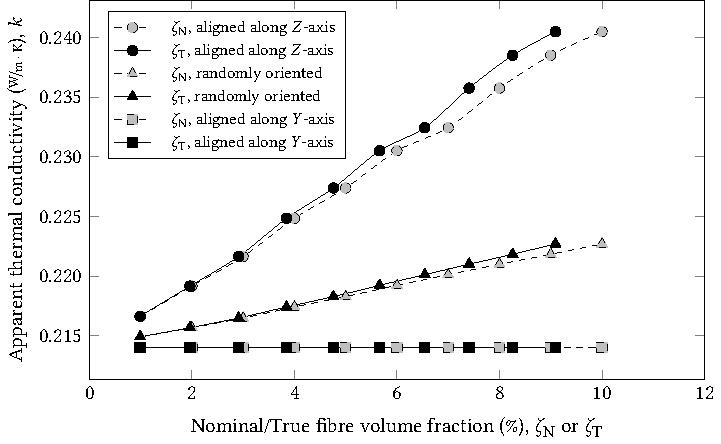
\includegraphics[scale=1]{chap4_res}
\caption{Results of the simulations based on 20 repetitions per fibre volume fraction}\label{figure:ddf2_res1}
\end{figure}%
	
	The LN model has shown to produce reliable results in predicting the effective thermal conductivity of CNTs, see~\autocite{Kostagiannakopoulou.2016,Zimmer.2012}. To validate the FE model, the LN model is used as a benchmark for both aligned and randomly-oriented fibre. If the nominal fibre volume fraction is used in the model (LN-N), the FE results of the aligned distribution show a maximum of 12.16\% error whereas by using the true fibre volume fraction (LN-T), the error seems to be about 10\%. By increasing the fibre volume fraction, the error in both cases decrease. Although, true fibre volume fractions show better results, the error of both LN-N and LN-T models are of the same order of magnitude. 
	
	A similar discussion is valid for the case of randomly-oriented fibres except that the errors grow further towards 20\%. This can be attributed to the randomness of the meso-structure, which cannot be completely captured by merely analytical models. Comparing the error values to a previous study in~\autocite{Javanbakht.2016}, the algorithm here shows superior results because of implementing the periodicity of fibre distribution and removing the resin-rich areas.

	Fibres were added with random orientation, aligned along the heat flow (along the $Z$-axis), and perpendicular to the direction of the heat flow (along the $Y$-axis), see Table~\ref{table:ddf2_result}. A 12.37\% improvement in the average effective conductivity of the composite is obtained by adding 10\% aligned fibres along the $Z$-axis whereas along the $Y$-direction no improvement is observed, i.e., the conductivity of the reinforced matrix remains the same as that of the pure matrix. The latter result is because of representing fibres by 1D elements that lack any transverse properties. It is worth noticing that the results along the $Y$ axis are independent of the fibre volume fraction. However, such a perfect alignment is impractical and very small improvements should be observed.

\begin{table}[!h]
\centering\small
\caption{Simulation results of effective thermal conductivity for aligned and dispersed fibres for various fibre volume fractions}\label{table:ddf2_result}
\begin{tabular}{>{\centering}p{2.2cm}@{}>{\centering}p{2cm}@{}>{\centering}p{2cm}@{}>{\centering}p{2cm}@{}>{\centering}p{2cm}@{}>{\centering}p{2cm}@{}>{\centering\arraybackslash}p{2cm}}
\toprule
\multirow{3}{2.2cm}{\centering\arraybackslash\bfs{Nominal fibre volume fraction (\%)}}
& \multicolumn{3}{c}{\bfs{Average effective conductivity} ($\scriptscriptstyle\frac{\text{W}}{\text{m}\cdot\text{K}}$)}
& \multicolumn{3}{c}{\bfs{Improvement (\%)}}\\\cmidrule(l{0.2cm}r{0.2cm}){2-4}\cmidrule(l{0.2cm}r{0.2cm}){5-7}
& \bfs{Aligned along $Z$-axis}
& \bfs{Aligned along $Y$-axis}
& \multirow{2}{2cm}{\centering\arraybackslash\bfs{Dispersed}}
& \bfs{Aligned along $Z$-axis}
& \bfs{Aligned along $Y$-axis}
& \multirow{2}{2cm}{\centering\arraybackslash\bfs{Dispersed}}
\\\toprule
% aligned improvement 26.04%	25.24%	24.67%	26.02%	25.42%	25.85%	24.49%	25.01%	24.78%	23.83%
% dispersed 0.42%	0.78%	1.16%	1.59%	2.00%	2.44%	2.85%	3.27%	3.66%	4.06%
1 & 0.21663 & 0.21400 & 0.21490 & 1.23 & 0.0 & 0.42\\
2 & 0.21915 & 0.21400 & 0.21566 & 2.41 & 0.0 & 0.78\\
3 & 0.22163 & 0.21400 & 0.21648 & 3.57 & 0.0 & 1.16\\
4 & 0.22484 & 0.21400 & 0.21740 & 5.07 & 0.0 & 1.59\\
5 & 0.22738 & 0.21400 & 0.21827 & 6.25 & 0.0 & 2.00\\
6 & 0.23050 & 0.21400 & 0.21922 & 7.71 & 0.0 & 2.44\\
7 & 0.23243 & 0.21400 & 0.22011 & 8.61 & 0.0 & 2.85\\
8 & 0.23575 & 0.21400 & 0.22099 & 10.16& 0.0 & 3.27\\
9 & 0.23851 & 0.21400 & 0.22182 & 11.45& 0.0 & 3.66\\
10& 0.24048 & 0.21400 & 0.22269 & 12.37& 0.0 & 4.06\\\bottomrule
\end{tabular}
\end{table}%

	On the other hand, the randomly-oriented fibres demonstrate slight improvements in the equivalent thermal conductivity---a maximum of 4.06\% in the highest fibre volume fraction. Obviously, the amount of improvement seems to depend on the magnitude of the fibre volume fraction and is lower than what is observed when fibres are perfectly aligned along the heat flow direction. It is interesting to notice that the fibres aligned along the $Z$-axis were about three times more efficient than the random case. Thus by assuming a normal distribution of orientation, it could be concluded that the randomly oriented fibres in this study had an efficiency of almost 30\% in every direction.
	
	One should note the special behaviour of the thermal link elements (type 36 1D rods) in mimicking highly anisotropic properties. A fibre that is represented by this element type only reinforces the properties along its direction while disregarding any transverse properties. Such behaviour is very close to the high contrast anisotropic properties of the CNTs, see~\autocite{Savvas.2016}. It is experimentally proven that the reinforcing effect of CNTs loses its efficiency in randomly oriented arrangement, see~\autocite{Savvas.2016b}. Therefore, it seems that the selection of this element type and the outcome of the study are along the reported results in the literature. A comparison between the results of various element types is available in~\autocite{Yuan.2014}.
\bl

\section{Conclusions}
In this study, three cases of random fibre dispersion was considered by implementing the EET: aligned parallel to the boundary conditions (along the $Y$-axis), aligned perpendicular to the boundary conditions (along the $Z$-axis), and randomly dispersed fibres. The generation of short fibres was done by means of Fortran subroutines and a Python script. The simulations were repeated 20 times for each case and the average results investigated. The periodicity condition was also considered to improve the results. The higher fibre volume fraction made the FE model more sensitive to the mesh density in terms of the effective thermal conductivity. In addition, adding short fibres to the matrix increased the thermal conductivity of the composite in both cases of random dispersion and aligned along the $Z$-axis---for a maximum relative value of 12.37\% and 4.06\%, respectively.\red\ Namely, an efficiency of 30\% could be assigned to the randomly-oriented fibres. In contrast, no improvement was observed for the aligned case along the $Y$-axis. Furthermore, it was shown that the deviation between the nominal fibre volume fraction and its true counter part could inject errors in the results of analytical models and the output of the numerical algorithms. Such errors could increase for higher volume of fibres. It can be concluded that the optimised direction of the short fibres is along the temperature gradient while random distribution provides improvement to some extent but at almost every direction. 

The EET seems to be a convenient method for generating acceptable RVEs. The improved algorithm produced better result than its preceding version. However, the geometrical issues regarding the overlapping of the fibre and matrix volumes should be taken into consideration. Such issues vary depending on the type of elements that is used for each component of the composite and the type of analysis, e.g., thermal or mechanical. In this study, it was shown that the deviation of the true fibre volume fraction values from the nominal ones might become highly pronounced in high volume fractions, which may be of importance in critical calculations. In future studies, other geometrical issues that arise in the calculation of the apparent/effective thermal properties should also be considered.\bl

